\documentclass{article}

\usepackage{hyperref}
\usepackage{amsmath}
\usepackage{bm}
\usepackage{amssymb}
\usepackage{amsfonts}
\usepackage{amstext}
\usepackage{graphicx}

\title{\textbf{Six DOF Aircraft Simulator}}

\begin{document}

\maketitle

\section{Introduction}
The goal of this project is to implement a six degrees of freedom (DOF), nonlinear simulation for fixed-wing aircraft. 
The first iteration of this project is using a linear aircraft model. The second iteration will be using a nonlinear model. 
   
\section{Aircraft Model}
The linear longitudinal and lateral models for a conventional fixed-wing aircraft could be written as follows \cite{Nelson}.

\begin{equation} \label{Eq:Linear_Long_sys}
    \begin{bmatrix}
    \dot{u} \\
    \dot{w} \\
    \dot{q} \\
    \dot{\theta} \\ 	
    \end{bmatrix}
    =
    \begin{bmatrix}
    X_u & X_w & 0 & -g \cos{\theta_0}\\
    Z_u & Z_w & u_0 & -g \sin{\theta_0}\\
    M_u & M_w & M_q & 0\\
    0 & 0 & 1 & 0 \\
    \end{bmatrix}
    \begin{bmatrix}
    u \\
    w \\
    q \\
    \theta \\ 	
    \end{bmatrix}
    +
    \begin{bmatrix}
    X_{\delta_e} & X_{\delta_t} \\
    Z_{\delta_e} & 0 \\
    M_{\delta_e} & M_{\delta_t} \\
    0 & 0\\ 	
    \end{bmatrix}
    \begin{bmatrix}
    {\delta_e} \\
    {\delta_t}  	
    \end{bmatrix}
\end{equation}

\begin{equation} \label{Eq:Linearized_sys}
    \begin{bmatrix}
    \dot{v} \\
    \dot{p} \\
    \dot{r} \\
    \dot{\phi} \\
    \dot{\psi} \\
    \end{bmatrix}
    =
    \begin{bmatrix}
    Y_v & Y_p & -(u_0 - Y_r) & g \cos{\theta_0} & 0\\
    \mathcal{L}_v & \mathcal{L}_p & \mathcal{L}_r & 0 & 0\\
    N_v & N_p & N_r & 0 & 0\\
    0 & 1 & 0 & 0 & 0\\
    0 & 0 & \sec{\theta_0} & 0 & 0\\
    \end{bmatrix}
    \begin{bmatrix}
    v\\
    p\\
    r\\
    \phi\\
    \psi\\ 	
    \end{bmatrix}
    +
    \begin{bmatrix}
    0 & Y_{\delta_r} \\
    \mathcal{L}_{\delta_a} & \mathcal{L}_{\delta_r} \\
    N_{\delta_a} & N_{\delta_r} \\
    0 & 0\\
    0 & 0\\ 	
    \end{bmatrix}
    \begin{bmatrix}
    {\delta_a} \\
    {\delta_r}  	
    \end{bmatrix}
\end{equation}

In this project we will consider the linear model of the aircraft "DELTA" given in \cite[PP. 561--563]{Mclean}
whose parameters are given as follows (at $U_0 = 75~ m/s$ and $\theta_0 = 2.7 ^\circ$)
\begin{equation}\label{Eq:DELTA_Params}
    \begin{split}
        m &= 300000 kg\\
        X_u &= -0.02\\
        X_w &= 0.1\\
        Z_u &= -0.23\\
        Z_w &= -0.634\\
        M_u &= -2.55*10^{-5}\\
        M_w &= -0.005\\
        M_q &= -0.61\\
        Y_v &= -0.078\\
        Y_p &= 0\\
        Y_r &= 0\\
        \mathcal{L}_v &= -0.086\\
        \mathcal{L}_p &= -1.0758\\
        \mathcal{L}_r &= 0.6334\\
        N_v &= 0.0037\\
        N_p &= -0.1121\\
        N_r &= -0.2569\\
        X_{\delta_e} &= 0.14\\
        Z_{\delta_e} &= -2.9\\
        M_{\delta_e} &= -0.64\\
        X_{\delta_t} &= 1.56\\
        M_{\delta_t} &= 0.0054\\
        Y_{\delta_r} &= 0.0065\\
        \mathcal{L}_{\delta_a} &= 0.46\\
        \mathcal{L}_{\delta_r} &= 0.1\\
        N_{\delta_a} &= 0.05\\
        N_{\delta_r} &= -0.21\\
    \end{split}
\end{equation}
where $\delta_t$ is considered to be from the trim thrust. 
As such, $\delta_t$ is allowed the between $1$ and $-0.56$ \cite{Hassan2016_JAST}.

\section{Algorithm Structure}


\section{Results}
In this simulation example, the aircraft is subject to both elevator and aileron sinusoidal inputs
 with an amplitude of $5$ degrees and a frequency of $\pi$ rad/s. Figures \ref{Fig:Translational_Velocities}, 
 \ref{Fig:Rotational_Velocities} and \ref{Fig:Attitude} show the resulting translational velocities, 
 rotational velocities and attitude angles, respectively.
\begin{figure}[h]
    \centering
    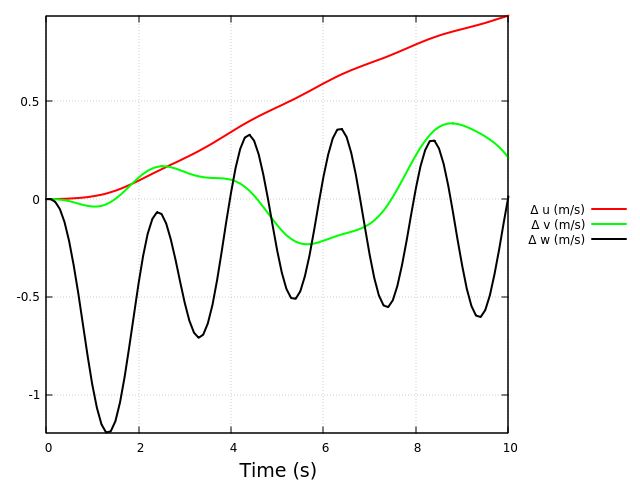
\includegraphics[width=0.9\textwidth]{sim_results_uvw.png}
    \caption{Translational velocities.}
    \label{Fig:Translational_Velocities}
\end{figure}
\begin{figure}[h]
    \centering
    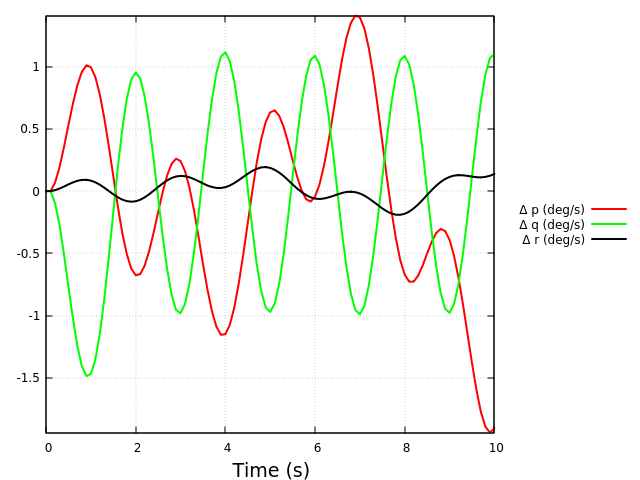
\includegraphics[width=0.9\textwidth]{sim_results_pqr.png}
    \caption{Rotational velocities.}
    \label{Fig:Rotational_Velocities}
\end{figure}
\begin{figure}[h]
    \centering
    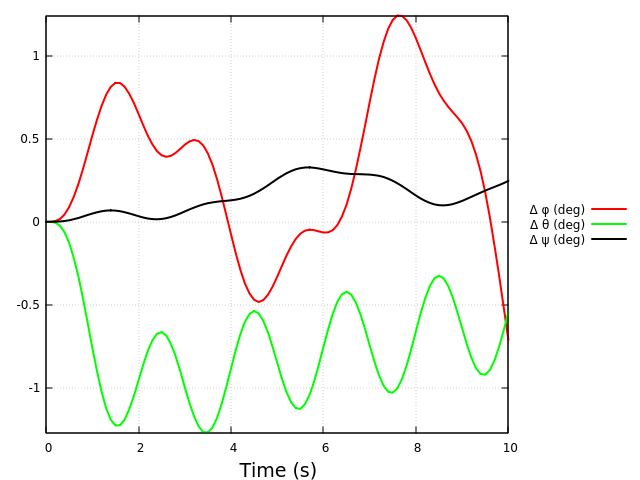
\includegraphics[width=0.9\textwidth]{sim_results_phi_theta_psi.png}
    \caption{Attitude angles.}
    \label{Fig:Attitude}
\end{figure}


\bibliographystyle{unsrt}
\bibliography{ref}
\end{document}